
\begin{frame}[t] 
\slidesonly{\frametitle{The mean-field approximation for pairwise clustering}}

\svspace{-3mm}

\begin{block}{assignment noise $\rightarrow$ Gibbs distribution}
$$
	P_{ \big( \big\{ m_q^{(\alpha)} \big\} \big) }
	= \frac{1}{Z_p} \exp \Big\{ -\beta 
	\overbrace{
		E_{\big[ \big\{ m_q^{(\alpha)} \big\} \big]}
		}^{= \, E_p}
		\Big\}
$$
where
$$
	Z_p = \sum\limits_{\mathscr{M}} \exp \Big\{ -\beta
		E_p
		\Big\}
$$
\end{block}
\notesonly{
This is approximated by the mean-fields:
}
\begin{block}{factorizing distribution}
$$
	Q_{ \big[ \big\{ m_q^{(\alpha)} \big\} \big] }
	= \frac{1}{Z_Q} \exp \Big\{ -\beta \sum\limits_{q, \gamma}
		m_q^{(\gamma)} \underbrace{ e_q^{(\gamma)} }_{
			\text{{\tiny mean-fields}} } \Big\}
$$
where:
$$
	Z_Q = \sum\limits_{\mathscr{M}} \exp \Big\{ -\beta \sum\limits_{q, 
		\gamma} m_q^{(\gamma)} e_q^{(\gamma)} \Big\}
$$
\end{block}
\end{frame}

\begin{frame}\frametitle{Recap calculation of the moments (general mean-field case)}
The factorization of the distribution $Q$ simplifies the calculation of the moments. 
This is based on the individual state variables being \emph{uncorrelated}.

\begin{equation}\label{eq:factorizingMoments}
	\Big< f_{(\vec{s}/s_l)} g_{(s_l)} \Big>_Q
	 = \frac{1}{Z_Q} \sum\limits_{\vec{s}} f_{(\vec{s}/s_l)}
		g_{(s_l)} \exp \Big( -\beta \sum\limits_k e_k s_k \Big)
\end{equation}

\end{frame}
\begin{frame}
\slidesonly{
\frametitle{Factorizing moments (general mean-field case)}
\vspace{-0.5cm}
\begin{equation}\label{eq:factorizingMoments}
	\Big< f_{(\vec{s}/s_l)} g_{(s_l)} \Big>_Q
	 = \frac{1}{Z_Q} \sum\limits_{\vec{s}} f_{(\vec{s}/s_l)}
		g_{(s_l)} \exp \Big( -\beta \sum\limits_k e_k s_k \Big)
\end{equation}
}
\begin{eqnarray*}
	& = & \frac{1}{Z_Q} \bigg[ \sum\limits_{\vec{s}/s_l} f_{(\vec{s}/s_l)}
		\exp \Big( -\beta \sum\limits_{k \neq l} e_k s_k \Big) \bigg]
		\bigg[ \sum\limits_{s_l} g_{(s_l)} \exp \Big( -\beta e_l
			s_l \Big) \bigg] \\\\
	& = & \frac{1}{Z_Q} \bigg[ \sum\limits_{\vec{s}/s_l} f_{(\vec{s}/s_l)}
		\exp \Big( -\beta \sum\limits_{k \neq l} e_k s_k \Big) \bigg]\\
		&&\qquad\qquad
  \frac{\color{blue}{\sum\limits_{s_l} \exp(-\beta e_l s_l)}}{\sum\limits_{s_l}
		\exp(-\beta e_l s_l)}
		\bigg[ {\color{blue}\sum\limits_{s_l}} g_{(s_l)} \color{blue}{\exp \Big( -\beta e_l
			s_l \Big)} \bigg] \\\\
	& = &\big< f_{(\vec{s}/s_l)} \big>_Q \frac{\sum\limits_{s_l}
		g_{(s_l)} \exp(-\beta e_l s_l)}{\sum\limits_{s_l}
		\exp(-\beta e_l s_l)} = 
	\underbrace{ \big< f_{(\vec{s}/s_l)} \big>_Q \cdot \big<g_{(s_l)} 
		\big>_Q }_{ 	\substack{ \text{factorization of moments} \\
				\rightarrow \text{uncorrelated variables}} }
\end{eqnarray*}

\end{frame}

\begin{frame}
\slidesonly{\frametitle{Calculation of moments}}
$$
		\begin{array}{lll}
	\big< m_q^{(\gamma)} \big>_Q
	& = \frac{1}{Z_Q} \sum\limits_{\mathscr{M}} m_q^{(\gamma)}
		\exp \Big\{ -\beta \sum\limits_{r, \delta} 
		m_{r}^{(\delta)} e_{r}^{(\delta)} \Big\}
	\end{array}
$$

\begin{itemize}
\itr The factorization of $Q$ simplifies the calculation of the moments.
\end{itemize}

\end{frame}

\begin{frame}
\slidesonly{\frametitle{Calculation of moments (derivation)}
The factorization in \eqref{eq:factorizingMoments}) regarding valid assignments $\big\{ \vec{m}^{(\gamma)} \big\}$ for observation $\gamma$ and the rest of the variables excluding $\gamma$ (i.e. $\mathscr{M}_{\gamma}$) is valid for any functions $f,g$:
}
\begin{align}
	\sum\limits_{\mathscr{M}} \Big[ f_{ \big( \big\{ m_p^{(\delta)} 
		\big| \delta \neq \gamma \big\} \big) }
		\cdot \, g_{ \big( \big\{ m_p^{(\delta)} \big| \delta = \gamma 
			\big\} \big) }
		\Big]\\
		\qquad
	\qquad\qquad= \Big[ \sum\limits_{\mathscr{M}_{\gamma}} f_{ \big( \big\{ 
		m_p^{(\delta)} \big| \delta \neq \gamma \big\} \big) }
		\Big] \cdot \Big[ \sum\limits_{\big\{ \vec{m}^{(\gamma)} 
			\big\} } g_{ \big( \big\{ m_p^{(\delta)} \big| \delta = 
			\gamma \big\} \big) } \Big]
\end{align}
this gives
%% this formula has been seriously confusing / wrong (indices?) so double check
\begin{equation}
	\begin{array}{ll}
	\big< m_q^{(\gamma)} \big>_Q
	& = \frac{ \Bigg[ \sum\limits_{\mathscr{M}_{\gamma}} \exp \Big\{ -\beta
		\sum\limits_{r, \delta \neq \gamma} m_{r}^{(\delta)}
		e_{r}^{(\delta)} \Big\} \Bigg] \cdot \Bigg[ 
		\overbrace{ \sum\limits_{ \big\{ \vec{m}^{(\gamma)} \big\} }
		m_q^{(\gamma)} }^{\substack{	\text{only term with} \\
						m_q^{(\gamma)} = 1 \\
						\text{remains} }}
		\exp \Big\{ -\beta \sum\limits_{r} m_{r}^{(\gamma)}
		e_{r}^{(\gamma)} \Bigg] }{
			\underbrace{
			\Bigg[ \sum\limits_{\mathscr{M}_{\gamma}} \exp 
			\Big\{ -\beta \sum\limits_{r, \delta \neq \gamma} 
			m_{r}^{(\delta)}e_{r}^{(\delta)} \Big\} \Bigg]
			}_{ \text{first terms cancel} } 
			\cdot \Bigg[ \sum\limits_{ \big\{ \vec{m}^{(\gamma)} 
			\big\} } \exp \Big\{ -\beta
			\underbrace{ \sum\limits_{r} m_{r}^{(\gamma)}
				e_{r}^{(\gamma)} }_{
				\substack{	\text{only one term of this} \\
						\text{sum remains for every} \\
						\text{term of the qrevious }
						\text{sum}} }
				\Big\} \Bigg] } \\\\
	 & = \frac{ \exp \big\{ -\beta\, m_q^{(\gamma)} e_q^{(\gamma)} \big\} }{
	 	\sum\limits_{r} \exp \big\{ -\beta \,
	 	m_{r}^{(\gamma)} e_{r}^{(\gamma)} \big\} }
	\; \underbrace{=}_{\substack{\text{only the } \\ m_r^{(\gamma)} = 1 \\\text{ stays}}} \; \underbrace{\frac{ \exp \big\{ -\beta e_q^{(\gamma)} \big\} }{
		\sum\limits_{r} \exp \big\{ -\beta 
		e_{r}^{(\gamma)} \big\} }}_{\text{soft-max of the mean-fields}}
	\end{array}
\end{equation}
\end{frame}

\begin{frame}
\frametitle{Solution for calculating the moments}
$$
		\begin{array}{lll}
	\big< m_q^{(\gamma)} \big>_Q
	& = \frac{ \exp \big\{ -\beta\, m_q^{(\gamma)} e_q^{(\gamma)} \big\} }{
	 	\sum\limits_{r} \exp \big\{ -\beta \,
	 	m_{r}^{(\gamma)} e_{r}^{(\gamma)} \big\} }
	\; = \underbrace{\;\; \frac{ \exp \big\{ -\beta e_q^{(\gamma)} \big\} }{
		\sum\limits_{r} \exp \big\{ -\beta 
		e_{r}^{(\gamma)} \big\} }\;\;}_{\text{soft-max of the mean-fields}}
	\end{array}
$$
\begin{block}{Intuition for above result: ``soft'' clustering}
\begin{itemize}
\itr $\sum_r \langle m_r^{(\gamma)} \rangle = 1$  and $\big< m_q^{(\gamma)} \big>_Q \in [0, 1]$ => assignment probabilities
\itr $\beta \rightarrow \infty: \big< m_q^{(\gamma)} \big>_Q \in \{0, 1\} $ => ``hard assignments'' (cmp.\ K-means)
\end{itemize} 
\end{block}
\end{frame}

\subsection{Soft clustering}

\begin{frame}{\subsecname}

\notesonly{
We have so far considered the case of assigning each data point to exactly \textbf{one} cluster. This is enforced by having used a binary definition for 
the assignments variables $m_q^{(\alpha)}$. This ``hard'' assignment is relaxed leading to a so-called ``soft'' or ``fuzzy'' assignment. 
}
Each data point $\vec x^{(\alpha)}$ is assigned to \textbf{all} clusters simultaneously but with different strengths:
The definition of the assignment variable for some point $\alpha$ becomes:
\begin{equation}
\label{eq:assignvarsoft}
\big< m_q^{(\alpha)} \big> \in [0, 1]
\end{equation}
such that
\begin{equation}
\label{eq:assignvarsoftnormalize}
\sum_{q=1}^{M}\big< m_q^{(\alpha)} \big> = 1.
\end{equation}

\notesonly{
The normalization in \eqref{eq:assignvarsoftnormalize} ensures that point $\alpha$ is completly assigned and allows us to interpret the assignment variables as \emph{assignment probabilities. See Fig\ref{fig:clusteringsoft}} for an example. 
The purpose of defining the assignment probabilities as ``expectations'' $\big< \cdot \big>$ will be clarified, when we discuss the soft clustering algorithm.
}
\begin{figure}[h!]
  \centering
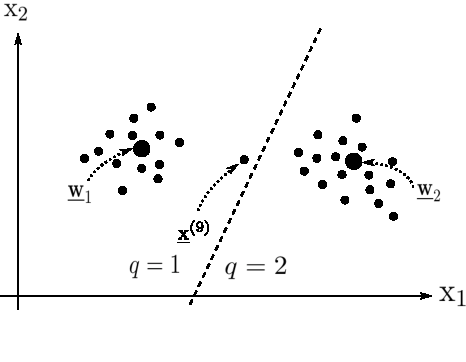
\includegraphics[height=4cm]{img/clustering_soft} 
  \caption{Example for soft clustering. Point (9) is assigned to cluster $1$ with a higher probability than to cluster 2: $\big< m_1^{(9)} \big> = 0.51$, $\big< m_2^{(9)} \big> = 0.49$}
  \label{fig:clusteringsoft}
\end{figure}
\end{frame}

\notesonly{

Going back to mean-field approximation:

The approximation is achieved by minimizing the KL-divergence between the distribution $P$ and $Q$. 
}

\begin{frame}[t] \slidesonly{\frametitle{Minimization of the KL-divergence}}
\begin{block}{Mean Field equation (c.f. section on Stochastic Optimization for how to arrive at this result)}
$$
	\fbox{$ \frac{\partial}{\partial e_l}\big<E_p\big>_Q 
		- \sum\limits_k e_k \frac{\partial}{\partial e_l} \big<s_k\big>_Q = 0
	$}
$$
\end{block}
$$	\frac{\partial \big< E_p \big>_Q}{\partial e_q^{(\alpha)}}
	- \sum\limits_{r, \gamma} \frac{
		\overbrace{ \partial \big< m_r^{(\gamma)} \big>_Q }^{
			\substack{	\text{depends only on} \\
					\text{data point } \gamma }}}{
			\partial e_q^{(\alpha)}}
		e_r^{(\gamma)} \eqexcl 0
$$
$$
	\frac{\partial \big< E_p \big>_Q}{\partial e_q^{(\alpha)}}
	- \sum\limits_r \frac{\partial \big< m_r^{(\alpha)} \big>_Q}{
		\partial e_q^{(\alpha)}}
		e_r^{(\alpha)} \eqexcl 0
$$

switch to lecture slides....
\end{frame}
